\documentclass[a4paper,titlepage,12pt]{article}
\usepackage[utf8]{inputenc} %Make sure all UTF8 characters work in the document
%\usepackage{color}
\usepackage{graphicx}
\usepackage{titling}
%\usepackage{tabularx}
%\usepackage{longtable}
\usepackage[yyyymmdd]{datetime}
\usepackage[figurename=Figur]{caption}
\usepackage{booktabs}

%Set page size
\usepackage{geometry}
\geometry{margin=3cm}

\renewcommand{\dateseparator}{-}
\renewcommand{\contentsname}{Innehållsförteckning}

%%%%%%%%%%%%%%%%%%%%%%%%%%%%%%%
% Header and footer
%%%%%%%%%%%%%%%%%%%%%%%%%%%%%%%
\usepackage{fancyhdr}
\pagestyle{fancy}

\lhead{\includegraphics[width=0.15\linewidth]{../images/logo_full.png}}
\chead{Systemskiss för sexbent robot}
\rhead{\today}
\setlength\headheight{26pt} 

\lfoot{TSEA29 --- KMM \\ LIPS Systemskiss}
\rfoot{Grupp 9 \\ LiTHe Hex}

\newcommand{\itc}{I\textsuperscript{2}C}

\pretitle{%
    \begin{center}
        \LARGE
        \includegraphics[width=6cm]{../images/logo_full.png}\\[\bigskipamount]
}

\posttitle{\end{center}}

\begin{document}
    \title{\LARGE
        \textbf{Systemskiss för sexbent robot} \\
        \vspace*{0.5\baselineskip}
        \large
        Redaktör Frans Skarman \\
        Grupp 9 \\
        \small
        \vspace*{0.5\baselineskip}
        Version 0.1}

    \date{\today}

	\maketitle
	
	\newpage
	
	\begin{center}

		%%%%%%%%%%%%%%%%%%%%%%%%%%%%%%%%%%%%%%%%%%%%%%%%%%%%%%%%%%%%%%%%%%%%%%%%%%%%%%%%%
		%						Medlemmar
		%%%%%%%%%%%%%%%%%%%%%%%%%%%%%%%%%%%%%%%%%%%%%%%%%%%%%%%%%%%%%%%%%%%%%%%%%%%%%%%%%

		\section*{Projektidentitet}
		Grupp 9, Ht 2016, LiTHe Hex

		Linköpings Tekniska Högskola, ISY

		\begin{table}[h]
			\begin{center}
				\begin{tabular}[pos]{ l l l }
					\textbf{Namn} & \textbf{Ansvar} & \textbf{E-post} \\ \midrule
					Emil Segerbäck & Webbgränssnitt & emise935@student.liu.se \\ \midrule
					Frans Skarman & Dokumentansvarig & frask812@student.liu.se \\ \midrule
					Hannes Tuhkala & & hantu447@student.liu.se \\ \midrule
					Malcolm Vigren & Projektledare & malvi108@student.liu.se \\ \midrule
					Noak Ringman &  & noari093@student.liu.se \\ \midrule
					Olav Övrebö &  & olaov121@student.liu.se \\ \midrule
					Robin Sliwa &  & robsl733@student.liu.se \\
				\end{tabular}
			\end{center}
		\end{table}

		\centering
		\textbf{Kursansvarig}: Tomas Svensson Rum 3B:528 013--28 13 68 tomas.svensson@liu.se

		\newpage
		\tableofcontents
		\newpage


		%%%%%%%%%%%%%%%%%%%%%%%%%%%%%%%%%%%%%%%%%%%%%%%%%%%%%%%%%%%%%%%%%%%%%%%%%%%%%%%%%
		%						Historik
		%%%%%%%%%%%%%%%%%%%%%%%%%%%%%%%%%%%%%%%%%%%%%%%%%%%%%%%%%%%%%%%%%%%%%%%%%%%%%%%%%

		\section*{Dokumenthistorik}
		\begin{table}[h]
			\begin{tabular}[pos]{ l l l l l }
				\textbf{Version} & \textbf{Datum} & \textbf{Utförda förändringar} 
				& \textbf{Utförda av} & \textbf{Granskad} \\ \midrule

				0.1 & 2016--09--09 & Första utkastet & Projektgruppen & \\

			\end{tabular}
		\end{table}
	\end{center}

	%%%%%%%%%%%%%%%%%%%%%%%%%%%%%%%%%%%%%%%%%%%%%%%%%%%%%%%%%%%%%%%%%%%%%%%%%%%%%%%%%
	%						Inledning
	%%%%%%%%%%%%%%%%%%%%%%%%%%%%%%%%%%%%%%%%%%%%%%%%%%%%%%%%%%%%%%%%%%%%%%%%%%%%%%%%%

	\newpage

	\section{Inledning}
	I detta dokument beskrivs delsystemen mer ingående samt förslag på hur de ska implementeras.
	De delsystem som roboten ska använda sig av är:
	Centralenhet, motorikenhet och sensorenhet.

	%%%%%%%%%%%%%%%%%%%%%%%%%%%%%%%%%%%%%%%%%%%%%%%%%%%%%%%%%%%%%%%%%%%%%%%%%%%%%%%%%
	%						Översikt
	%%%%%%%%%%%%%%%%%%%%%%%%%%%%%%%%%%%%%%%%%%%%%%%%%%%%%%%%%%%%%%%%%%%%%%%%%%%%%%%%%

  \newpage
	\section{Systemöversikt}
	Systemet ska innehålla tre enheter. En centralenhet för kommunikation med en
    dator, en motorikenhet som sköter hur benen rör sig samt en sensorenhet som
    tolkar sensordata. Centralenheten är även den enhet som tar beslut och
    kommunicerar med de andra enheterna. Se Figur.~\ref{fig:overview} för en översiktsbild av
    systemet.
	\begin{figure}[h]
		\centering
		\includegraphics[width=0.5\linewidth]{../images/overview.png}
		\caption{Översikt av systemet\label{fig:overview}}
	\end{figure}

	\subsection{Kommunikation mellan enheterna}
	Kommunikation kan ske med UART, SPI eller \itc{}. AVR-processorerna har
	2 UART-, 3 SPI- och en \itc{}-ingång medan Raspberry PI:en har 1 UART-, 2 SPI- och
	en \itc{}-ingång. 

	\subsubsection{Förslag 1}
	Om vi vill ha en LIDAR-avståndsmätare kommer sensorenhetens \itc{}-port att gå åt
	till kommunikation med avståndsmätaren. Sensorenheten måste alltså kommunicera med
	centralenheten via UART eller SPI. Om kommunikationen sker med UART måste 
	motorikenheten kommunicera med SPI eftersom att centralenheten endast har en
	UART port.

	\subsubsection{Förslsag 2}
	Om både motorikenheten och sensorenheten har sin \itc{} buss tillgänglig kan 
	kommunikationen mellan de tre enheterna ske via en gemensam \itc{} buss där
	centralenheten är master och de andra enheterna är slavar. 
	
	
	
	\subsection{Grov beskrivning av systemet}
	Här var det text här var det text här var det text
	här var det text här var det text här var det text
	här var det text här var det text här var det text.
	
	
	\subsection{Ingående delsystem}
	Här var det text här var det text här var det text
	här var det text här var det text här var det text
	här var det text här var det text här var det text.
	
	
	\section{Centralenheten}
	Centralenheten har 4 huvudsyften: navigation/beslutsfattning, hinderdetektion samt
	kommunikation med omvärlden.

	\subsection{Navigation och beslutsfattning}

	\subsection{Hinderdetektion}
	För hinderdetektering finns det olika alternativ att använda. Det är möjligt att 
	detektera hinder medhjälp av en avståndsmätare som är vinklad nedåt, en IR sensor 
	eller LIDAR laser kan användas som avståndsmätare. Använda en IR sensor är enklast 
	eftersom IR sensorer antagligen kommer att användas för att undvika väggar. En 
	LIDAR laser är en ny enhet och använder ett mer avancerat gränssnitt I2C än 
	analog för IR. Ett annat alternativ för att upptäcka hinder är att läsa av det 
	motstånd som benens servo kan returnera tillsammans med övriga sensorer för 
	att upptäcka när roboten går in i ett hinder. 

	\subsection{Kommunikation}
	Centralenheten ska kommunicera med en dator över WiFi. Det är datorns webbläsare 
	som kommer att ansluta till centralenhetens webbserver, det blir då möjligt att 
	styra samt logga roboten via webbgränssnittet. Det finns flera gränssnitt att 
	använda för kommunikation mellan processorerna, intressanta gränssnitt är SPI, 
	I2C och UART. UART är inte möjligt att använda till sensorenheten och 
	motorikenheten på grund av att Raspberry Pi endast har en UART port. Både 
	SPI och I2C är möjligt att använda sätt till portar på alla enheterna sålänge 
	sensorenheten inte använder LIDAR laser, LIDAR laser använder I2C och endast en 
	I2C port finns på sensorenheten. I2C måste konfigureras med ett master/slave 
	förhållande. Centralenheten behöver vara master för att kunna kommunicera med 
	sensorenheten och motorikenheten som är slave. Med den konfigurationen blir 
	det inte möjligt för sensorenhet och motorikenheten att kommunicera med
	centralenheten utan att centralenheten har på startat kommunikationen. I och 
	med att I2C behöver en master/slave konfiguration blir SPI enklare att använda 
	för tvåvägskommunikation. 



	%%%%%%%%%%%%%%%%%%%%%%%%%%%%%%%%%%%%%%%%%%%%%%%%%%%%%%%%%%%%%%%%%%%%%%%%%%%%%%%%%
	%						Motorikenheten
	%%%%%%%%%%%%%%%%%%%%%%%%%%%%%%%%%%%%%%%%%%%%%%%%%%%%%%%%%%%%%%%%%%%%%%%%%%%%%%%%%
	
	\section{Motorikenheten}
	Här var det text här var det text här var det text
	här var det text här var det text här var det text
	här var det text här var det text här var det text.
	
	
	%%%%%%%%%%%%%%%%%%%%%%%%%%%%%%%%%%%%%%%%%%%%%%%%%%%%%%%%%%%%%%%%%%%%%%%%%%%%%%%%%
	%						Sensorenheten
	%%%%%%%%%%%%%%%%%%%%%%%%%%%%%%%%%%%%%%%%%%%%%%%%%%%%%%%%%%%%%%%%%%%%%%%%%%%%%%%%%
	\section{Sensorenheten}
    
    Sensorenheten är den enhet som ger roboten sinnen för omvärlden, så att den
    kan navigera autonomt 

    \subsection{Styrenhet}

    \subsection{Gyro}
    
    \subsection{Avståndssensorer i sidled}


\end{document}
